%%%%%%%%%%%%%%%%%%%%%%%%%%%%%%%%%%%%%%%%%%%%%%%%%%%%%%%%%%%%%%%%%%%%%%%%%%%%%%%
%% SOCIOL 723 -- Social Statistics II
% Week 6 -- Matching, Propensity Scores, and Weighting
%% Wenhao Jiang, Duke University, Fall 2026
%%%%%%%%%%%%%%%%%%%%%%%%%%%%%%%%%%%%%%%%%%%%%%%%%%%%%%%%%%%%%%%%%%%%%%%%%%%%%%%

\documentclass[aspectratio=169,11pt,xcolor=dvipsnames]{beamer}
\mode<presentation>

%% ---- fonts: Latin Modern Roman (the LaTeX default), serif throughout -------
\usepackage[T1]{fontenc}
\usepackage{lmodern}
\usefonttheme{serif}
\renewcommand{\familydefault}{\rmdefault}

%% ---- packages --------------------------------------------------------------
\usepackage{amsmath,amsfonts,amssymb,bm}
\usepackage{graphicx}
\usepackage{booktabs}
\usepackage{tikz}
\usetikzlibrary{arrows.meta,positioning,calc}
\usepackage[english]{babel}

\newcommand{\srcp}[1]{{\scriptsize\color{gray}(#1)}}
\newcommand{\srct}[1]{#1}

\DeclareMathOperator*{\argminop}{arg\,min}
\DeclareMathOperator*{\argmaxop}{arg\,max}
%% \limits forces the subscript underneath even in inline math
\newcommand{\argmin}{\argminop\limits}
\newcommand{\argmax}{\argmaxop\limits}
\DeclareMathOperator{\Cov}{Cov}
\DeclareMathOperator{\Var}{Var}
\DeclareMathOperator{\trace}{tr}
\DeclareMathOperator{\rank}{rank}
\DeclareMathOperator{\plim}{plim}
\newcommand{\indep}{\perp\!\!\!\perp}

%% ---- notation conventions (course-wide) ------------------------------------
\newcommand{\E}{E}
\newcommand{\En}{\mathbb{E}_n}
\newcommand{\R}{\mathbb{R}}
\newcommand{\X}{\bm{X}}
\newcommand{\Y}{\bm{y}}
\newcommand{\Ix}{\bm{I}}
\newcommand{\zero}{\bm{0}}
\newcommand{\bhat}{\hat{\bm{\beta}}}
\newcommand{\dto}{\overset{d}{\longrightarrow}}
\newcommand{\pto}{\overset{p}{\longrightarrow}}
\usetikzlibrary{shapes,decorations.pathmorphing}
\newcommand{\lik}{\mathcal{L}}
\newcommand{\loglik}{\ell}
\newcommand{\Info}{\mathcal{I}}
\newcommand{\SE}{\mathrm{se}}

%% ---- theme -----------------------------------------------------------------
\usetheme{default}
%% thin single-line header: clickable section names, current one highlighted.
%% (miniframes is deliberately not used: one dot per slide wraps to 4 rows here)
\setbeamerfont{section in head/foot}{size=\tiny}
\setbeamertemplate{headline}{%
  \begin{beamercolorbox}[wd=\paperwidth,ht=2.4ex,dp=1.1ex,%
                         leftskip=.3cm,rightskip=.3cm]{section in head/foot}%
    \usebeamerfont{section in head/foot}%
    \insertsectionnavigationhorizontal{.94\paperwidth}{}{}%
  \end{beamercolorbox}%
}

\definecolor{dukeblue}{RGB}{1,33,105}
\definecolor{accent}{RGB}{200,78,0}
\definecolor{softgray}{RGB}{242,242,245}

\setbeamercolor{structure}{fg=dukeblue}
\setbeamercolor{frametitle}{fg=dukeblue,bg=white}
\setbeamercolor{section in head/foot}{fg=white,bg=dukeblue}
\setbeamercolor{section in head/foot shaded}{fg=white!50!dukeblue,bg=dukeblue}
\setbeamercolor{alerted text}{fg=accent}
\setbeamercolor{block title}{fg=white,bg=dukeblue}
\setbeamercolor{block body}{fg=black,bg=softgray}
\setbeamercolor{block title alerted}{fg=white,bg=accent}
\setbeamercolor{block body alerted}{fg=black,bg=softgray}

\setbeamertemplate{footline}[page number]
\setbeamertemplate{navigation symbols}{}
%% continued frames keep the SAME font size and spill onto a new slide
\setbeamertemplate{frametitle continuation}{\normalfont\footnotesize\ (cont.)}
\setbeamertemplate{itemize items}[circle]
\setbeamertemplate{blocks}[rounded][shadow=false]
\setbeamerfont{frametitle}{series=\bfseries}
\setbeamerfont{footnote}{size=\scriptsize}
\setbeamerfont{caption}{size=\footnotesize}
\setbeamertemplate{subsection in head/foot}{}
\setbeamertemplate{subsection in head/foot shaded}{}
\setbeamertemplate{caption}[numbered]

\newcommand{\adv}{\,\raisebox{0.6pt}{\textcolor{accent}{$\bigstar$}}}

\setbeamertemplate{section page}{%
  \begin{centering}\vfill
  {\usebeamercolor[fg]{structure}\Large\bfseries\insertsectionhead\par}
  \vskip4pt{\color{dukeblue}\rule{0.35\linewidth}{1pt}\par}
  \vfill\end{centering}}
\setbeamertemplate{subsection page}{%
  \begin{centering}\vfill
  {\usebeamercolor[fg]{structure}\large\bfseries\insertsubsectionhead\par}
  \vfill\end{centering}}

\AtBeginDocument{%
  \setlength{\abovedisplayskip}{5pt}%
  \setlength{\belowdisplayskip}{5pt}%
  \setlength{\abovedisplayshortskip}{2pt}%
  \setlength{\belowdisplayshortskip}{3pt}%
}
\setbeamertemplate{frametitle}{%
  \vskip4pt\usebeamerfont{frametitle}\usebeamercolor[fg]{frametitle}%
  \insertframetitle\par\vskip2pt}
\setbeamersize{text margin left=0.75cm, text margin right=0.75cm}

%% ---- title -----------------------------------------------------------------
\title[SOCIOL 723]{SOCIOL 723: Social Statistics II\\[2pt]}
\subtitle{\large Week 6, Matching, Propensity Scores, and Weighting\\[-8pt]}
\author[Jiang]{\large Wenhao Jiang\vspace{-1.5em}}
\institute[Duke]{}
\titlegraphic{
\includegraphics[height=1.3cm]{../Misc/duke_logo.png}}
\date{\large Department of Sociology, Fall 2026}



\begin{document}

\begin{frame}[plain]
  \titlepage
\end{frame}

\begin{frame}{Today}
  \tableofcontents
\end{frame}

\begin{frame}{Where We Are}
Last week we established that under \textbf{conditional ignorability},
\textbf{positivity}, \textbf{consistency}, and \textbf{SUTVA},
\begin{align*}
  \text{ATE} = \E\Big[\,\E[Y_i\mid D_i=1,X_i] - \E[Y_i\mid D_i=0,X_i]\,\Big] .
\end{align*}
Today we take that identification result as \emph{given} and ask a purely
practical question: \alert{how should we actually do the adjustment?}
\vskip3pt
\begin{block}{Four answers, and they are more alike than they look}
\begin{enumerate}\itemsep1pt
  \item \textbf{Matching}: find comparison units that look like the treated ones.
  \item \textbf{Regression / g-computation}: model $\E[Y\mid D,X]$ and average.
  \item \textbf{Weighting}: reweight the sample so treatment is unrelated to $X$.
  \item \textbf{Doubly robust}: do both, and get insurance.
\end{enumerate}
\end{block}
\vskip2pt
All four estimate the \emph{same} identified quantity. They differ in what they
model, \alert{what weights they put on covariate cells}, what they extrapolate,
and how they fail.
\end{frame}

%%%%%%%%%%%%%%%%%%%%%%%%%%%%%%%%%%%%%%%%%%%%%%%%%%%%%%%%%%%%%%%%%%%%%%%%%%%%%%%
\section[Anatomy]{The Anatomy of Adjustment}
%%%%%%%%%%%%%%%%%%%%%%%%%%%%%%%%%%%%%%%%%%%%%%%%%%%%%%%%%%%%%%%%%%%%%%%%%%%%%%%
\begin{frame}\sectionpage\end{frame}

\begin{frame}{Cell-by-Cell Comparison}
Suppose $X_i$ takes finitely many values and write the cell-level effect
\begin{align*}
  \delta(X_i = x) \equiv \E[Y_i(1)-Y_i(0) \mid X_i = x]
  = \E[Y_i\mid D_i=1,X_i=x] - \E[Y_i\mid D_i=0,X_i=x] ,
\end{align*}
where the second equality is conditional ignorability.
\vskip3pt
Every method today is a choice of \alert{weights on $\delta(X_i=x)$}:
\begin{align*}
  \delta_{\text{ATE}} &= \sum_x \delta(X_i=x)\,\Pr(X_i = x) \\[2pt]
  \delta_{\text{ATT}} &= \sum_x \delta(X_i=x)\,\Pr(X_i = x \mid D_i = 1)
\end{align*}
\vskip2pt
The ATE weights cells by how common they are in the population; the ATT weights
them by how common they are \emph{among the treated}. Same ingredients,
different recipe.
\end{frame}

\begin{frame}{Anatomy of the Matching Estimand}
Apply Bayes' rule to the ATT weights:
\begin{align*}
  \Pr(X_i = x \mid D_i = 1)
  = \frac{\Pr(D_i = 1\mid X_i = x)\,\Pr(X_i=x)}{\Pr(D_i=1)} .
\end{align*}
\pause
Substituting,
\begin{align*}
  \boxed{\;
  \delta_{\text{ATT}}
  = \frac{\sum_x \delta(X_i = x)\;\Pr(D_i=1\mid X_i=x)\;\Pr(X_i=x)}
         {\sum_x \Pr(D_i=1\mid X_i=x)\;\Pr(X_i=x)}\;}
\end{align*}
\vskip3pt
\alert{The matching-based ATT weights each cell effect in proportion to the
probability of treatment in that cell}; that is, in proportion to the
propensity score $e(x)$. Cells where treatment is common count for more, which
is exactly what ``the effect on the treated'' should mean.
\end{frame}

\begin{frame}{Anatomy of Regression Adjustment: Setup}
Now do the same accounting for regression. To avoid conflating the weighting
question with a functional-form question, specify a model
\emph{saturated in $X_i$}:
\begin{align*}
  Y_i = \sum_x \mathbf{1}(X_i = x)\,\alpha_x \;+\; \delta_R\, D_i \;+\; \epsilon_i .
\end{align*}
\vskip3pt
By Frisch--Waugh--Lovell (Week 1), with $\check D_i \equiv D_i - \E[D_i\mid X_i]$
the residualized treatment,
\begin{align*}
  \delta_R
  = \frac{\Cov(Y_i,\check D_i)}{\Var(\check D_i)}
  = \frac{\E\big[\check D_i\, \E[Y_i \mid D_i, X_i]\big]}{\E\big[\check D_i^{\,2}\big]}
  = \frac{\E\big[(D_i - \E[D_i\mid X_i])\,\E[Y_i\mid D_i,X_i]\big]}
         {\E\big[(D_i-\E[D_i\mid X_i])^2\big]} .
\end{align*}
\vskip2pt
So the question becomes: what does the numerator simplify to?
\end{frame}

\begin{frame}{Anatomy of Regression Adjustment: the Numerator}
Because $D_i$ is binary, the conditional expectation decomposes exactly:
\begin{align*}
  \E[Y_i\mid D_i,X_i]
  &= \E[Y_i\mid D_i=0,X_i]
   + D_i\Big(\E[Y_i\mid D_i=1,X_i]-\E[Y_i\mid D_i=0,X_i]\Big) \\
  &= \E[Y_i\mid D_i=0,X_i] + D_i\,\delta(X_i) .
\end{align*}
\pause
Substitute into the numerator:
\begin{align*}
  &\E\Big[(D_i - \E[D_i\mid X_i])\big(\E[Y_i\mid D_i=0,X_i] + D_i\delta(X_i)\big)\Big] \\
  &\quad= \underbrace{\E\Big[(D_i-\E[D_i\mid X_i])\,\E[Y_i\mid D_i=0,X_i]\Big]}_{=\,0
     \text{ (a function of } X_i \text{ only)}}
   + \E\Big[(D_i-\E[D_i\mid X_i])\,D_i\,\delta(X_i)\Big] \\[2pt]
  &\quad= \E\Big[(D_i - \E[D_i\mid X_i])^2\,\delta(X_i)\Big] ,
\end{align*}
where the last step uses $\E[(D_i-\E[D_i\mid X_i])D_i \mid X_i]
= \Var(D_i\mid X_i)$.
\end{frame}

\begin{frame}{Anatomy of Regression Adjustment: the Result}
Putting numerator and denominator together and applying iterated expectations:
\begin{align*}
  \delta_R
  = \frac{\E\big[(D_i-\E[D_i\mid X_i])^2\,\delta(X_i)\big]}
         {\E\big[(D_i-\E[D_i\mid X_i])^2\big]}
  = \boxed{\;\frac{\E\big[\sigma_D^2(X_i)\,\delta(X_i)\big]}{\E\big[\sigma_D^2(X_i)\big]}\;}
\end{align*}
where $\sigma_D^2(x) \equiv \Var(D_i\mid X_i = x)$. Since $D_i$ is binary,
$\sigma^2_D(x) = e(x)\big(1-e(x)\big)$, so
\begin{align*}
  \delta_R = \frac{\sum_x \delta(X_i=x)\, e(x)\big(1-e(x)\big)\,\Pr(X_i=x)}
                  {\sum_x e(x)\big(1-e(x)\big)\,\Pr(X_i=x)} .
\end{align*}
\vskip2pt
\alert{Regression weights each cell by the \emph{conditional variance} of
treatment.} Compare with matching, which weighted by $e(x)$ itself. Cells with
$e(x)\approx 0.5$ dominate the regression, and cells that are nearly all treated
or nearly all control contribute almost nothing \emph{to $\delta_R$}. Matching
behaves differently at the top end, which is the next slide.
\end{frame}

\begin{frame}[allowframebreaks,t]{Two Consequences Worth Stating Plainly}
\begin{itemize}\itemsep4pt
  \item \textbf{The two weightings answer different questions} even under
        identical assumptions and with the same saturated specification. Matching
        is a \emph{method}, not an estimand, and can be pointed at the ATE or the
        ATT by changing the cell weights; the ATT weighting above is the one that
        necessarily differs from $\delta_R$. Neither $\delta_R$ nor the ATT is
        ``the'' ATE unless effects are homogeneous.
  \item \textbf{The regression weight $e(x)(1-e(x))$ vanishes at $e(x)\in\{0,1\}$},
        so cells with no comparison units drop out of $\delta_R$ silently.
        \alert{Positivity failures do not produce an error message; they produce a
        quietly redefined estimand.}
  \item Matching is different: a cell with $e(x)\approx1$ carries a \emph{large}
        ATT weight. But at $e(x)=1$ there is no control unit, so $\delta(x)$ is
        simply not identified; the estimator has nothing to average, and the
        honest response is to say which cells you dropped.
\end{itemize}
\vskip4pt
\begin{block}{With continuous covariates}
The anatomy still holds, as an integral:
\begin{align*}
  \delta_R = \frac{\int \delta(x)\,e(x)\big(1-e(x)\big)f(x)\,dx}
                  {\int e(x)\big(1-e(x)\big)f(x)\,dx} .
\end{align*}
\end{block}
\end{frame}

\begin{frame}{Regression as Fuzzy Matching}
With continuous $X$, exact common support at every $X_i = x$ is impossible in a
finite sample. Positivity becomes the requirement that $0 < e(x) < 1$ on the
support, so that in a \emph{neighbourhood} of any covariate value both treated
and untreated units occur:
\begin{align*}
  \E[Y_i(d)\mid X_i = x] = \lim_{\varepsilon\to 0}
  \E\big[Y_i(d) \mid X_i \in (x-\varepsilon, x+\varepsilon)\big] .
\end{align*}
\vskip3pt
\begin{itemize}\itemsep3pt
  \item In that sense, regression with continuous covariates \emph{is} a fuzzy
        matching method, giving the largest weights to neighbourhoods with the
        most balanced overlap.
  \item \alert{Without common support, regression still returns a number}, by
        extending the fitted control line into the treated region. That recovers
        the truth only if the control surface $\E[Y\mid D=0,X]$ is correctly
        specified out there \emph{and} the treatment effect is constant across
        $X_i$, two functional-form claims, neither checkable where there are no
        data.
  \item This is the deepest reason to look at overlap before running anything.
\end{itemize}
\end{frame}

\begin{frame}[allowframebreaks,t]{Does It Matter Empirically? Angrist (1998)}
Effect of \emph{voluntary} military service on 1988--91 Social Security earnings,
among men who applied to enter the armed forces 1979--82. Matching and regression
both control for year of birth, education at application, and AFQT score.
\begin{center}\small
\renewcommand{\arraystretch}{1.25}
\begin{tabular}{lccccc}
\toprule
 & Mean & Difference & Matching & Regression & Regression \\
 & earnings & in means & estimate & estimate & $-$ matching \\
\midrule
Whites & 14{,}537 & 1{,}233.4 & $-197.2$ & $-88.8$ & 108.4 \\
       &          & (60.3)    & (70.5)   & (62.5)  & (28.5) \\
Non-whites & 11{,}664 & 2{,}449.1 & 839.7 & 1{,}074.4 & 234.7 \\
       &          & (47.4)    & (62.7)   & (50.7)  & (32.5) \\
\bottomrule
\end{tabular}
\end{center}
\vskip3pt
{\footnotesize Adapted from Angrist (1998), Tables II and V. $n = 128{,}968$ whites,
$175{,}262$ non-whites.}
\vskip3pt
\begin{itemize}\itemsep1pt
  \item Adjustment reverses the sign for whites, selection into service is
        strongly positive on earnings potential.
  \item Matching and regression differ by about $100$--$235$ dollars, and the
        \emph{difference} is statistically significant. Small, but exactly the
        magnitude the weighting anatomy predicts.
\end{itemize}
\end{frame}
\section[Matching]{Matching}
%%%%%%%%%%%%%%%%%%%%%%%%%%%%%%%%%%%%%%%%%%%%%%%%%%%%%%%%%%%%%%%%%%%%%%%%%%%%%%%
\begin{frame}\sectionpage\end{frame}

\begin{frame}{The Idea, in Its Simplest Form}
Suppose $X_i$ takes finitely many values. For each cell $x$, compute the
difference in means, then average the cell-level differences with weights of your
choosing:
\begin{align*}
  \hat\tau_{\text{ATE}} = \sum_x \hat\Pr(X_i = x)\,
    \big[\bar Y_{1x} - \bar Y_{0x}\big],
  \qquad
  \hat\tau_{\text{ATT}} = \sum_x \hat\Pr(X_i = x \mid D_i = 1)\,
    \big[\bar Y_{1x} - \bar Y_{0x}\big] .
\end{align*}
\vskip4pt
\begin{itemize}\itemsep3pt
  \item This is \alert{exact matching}, and it is the cleanest possible
        implementation of ``compare like with like.''
  \item Notice: the only difference between the ATE and the ATT is
        \alert{the weights on the cells}. Choose them deliberately.
  \item Recall from Week 1 that OLS with a saturated $X$ reports its own
        variance-weighted average of the same cell effects. Matching lets you
        take the weights back.
  \item The catch: with more than a handful of covariates, most cells are empty.
\end{itemize}
\end{frame}

\begin{frame}[allowframebreaks,t]{The Curse of Dimensionality}
With $p$ binary covariates there are $2^p$ cells: $p=10$ gives 1{,}024, $p=20$
gives over a million. Exact matching becomes impossible long before the
covariates run out.
\vskip4pt
Practical responses, in rough order of desperation:
\begin{itemize}\itemsep3pt
  \item \textbf{Coarsened exact matching} (CEM): bin continuous covariates
        coarsely, age in five-year bands, income in quintiles, then match
        exactly on the bins. Transparent, and you see immediately what you had to
        discard.
  \item \textbf{Nearest-neighbour matching} on a distance: Euclidean, or
        \emph{Mahalanobis} $\big[(X_i - X_j)'\hat{\bm\Sigma}^{-1}(X_i - X_j)\big]^{1/2}$,
        which scales by the covariance so no variable dominates by its units.
  \item \textbf{Propensity score matching}: collapse $X$ to a single number, 
        the next section.
\end{itemize}
\vskip3pt
\alert{Every one of these is a way of admitting that exact comparisons run out in
\emph{your sample}.} That is finite-sample sparsity, which is not the same thing
as a structural positivity failure ($e(x)\in\{0,1\}$ in the population), though
in practice you often cannot tell them apart. Being explicit about where the
comparisons thinned is a feature.
\end{frame}

\begin{frame}[allowframebreaks,t]{Choices That Actually Matter}
\begin{itemize}\itemsep2pt
  \item \textbf{With or without replacement}. With replacement gives better
        matches and lower bias but higher variance, and the same control unit may
        be reused many times (which the standard errors must account for).
  \item \textbf{How many matches per treated unit}. More matches reduce variance
        and increase bias.
  \item \textbf{Calipers}. Refuse matches beyond some distance. This improves
        comparability but \alert{changes the estimand}: you are now describing
        whatever subpopulation survived.
  \item \textbf{Bias correction}. Nearest-neighbour matching on continuous
        covariates has a bias of order $n^{-1/p}$ that does not vanish fast
        enough; regress the residual difference on the covariate gap to remove it.
\end{itemize}
\vskip2pt
\begin{alertblock}{Report what matching discarded}
The number of treated units with no acceptable match is a substantive result. It
tells your reader exactly where the data cannot speak.
\end{alertblock}
\end{frame}

\begin{frame}{Matching Is Preprocessing, Not Estimation}
\srct{Ho, Imai, King, and Stuart (2007)} make the point that should organize your
workflow: matching is a \emph{nonparametric preprocessing step} that reduces how
much your final model has to do.
\vskip2pt
\begin{enumerate}\small\itemsep2pt
  \item Match, using \alert{no outcome data at all}. This is the design stage; it
        can be iterated freely without $p$-hacking, because you cannot see the
        answer.
  \item Check \textbf{balance}: are covariate distributions similar in the matched
        treated and control groups? Standardized mean differences below $0.1$,
        variance ratios near $1$, and eyeballed density overlaps.
  \item \emph{Then} run your regression on the matched sample. Any remaining
        imbalance is handled by the model, and because imbalance is now small,
        the answer is insensitive to how you specify it.
\end{enumerate}
\vskip2pt
{\small\alert{Never use a balance $t$-test.} Balance is a property of the sample you
have, not a hypothesis about a population. Its $p$-value depends on sample size,
so pruning observations makes it \emph{rise} through lost power even when
imbalance is unchanged: passing the test can mean you simply have less data
\srcp{Imai, King, and Stuart 2008}. Report standardized differences instead.}
\end{frame}

%%%%%%%%%%%%%%%%%%%%%%%%%%%%%%%%%%%%%%%%%%%%%%%%%%%%%%%%%%%%%%%%%%%%%%%%%%%%%%%
\section[Propensity Score]{The Propensity Score}
%%%%%%%%%%%%%%%%%%%%%%%%%%%%%%%%%%%%%%%%%%%%%%%%%%%%%%%%%%%%%%%%%%%%%%%%%%%%%%%
\begin{frame}\sectionpage\end{frame}

\begin{frame}{A Remarkable Theorem}
Define the \alert{propensity score}
\begin{align*}
  e(x) \equiv \Pr(D_i = 1 \mid X_i = x) .
\end{align*}
\begin{block}{Rosenbaum and Rubin (1983)}
If $\big(Y_i(0),Y_i(1)\big)\indep D_i \mid X_i$, then
\begin{align*}
  \big(Y_i(0),Y_i(1)\big)\indep D_i \mid e(X_i) .
\end{align*}
\end{block}
\vskip2pt
\begin{itemize}\itemsep2pt
  \item Conditioning on a \emph{single number} suffices. A $p$-dimensional
        matching problem collapses to a one-dimensional one.
  \item $e(X)$ is a \emph{balancing score}: within strata of $e(X)$, the whole
        covariate vector is distributed identically in the two groups.
  \item This is why the propensity score is everywhere. It is also why it is
        routinely oversold; it does nothing about \emph{unobserved}
        confounders.
\end{itemize}
\end{frame}

\begin{frame}{Proof of the Balancing Property\adv}
It suffices to show $\Pr(D_i = 1 \mid X_i, e(X_i)) = \Pr(D_i=1\mid e(X_i))$; the
left side is $e(X_i)$ by definition. For the right side, use iterated
expectations:
\begin{align*}
  \Pr\big(D_i = 1 \mid e(X_i)\big)
  = \E\big[\, \E[D_i \mid X_i] \ \big|\ e(X_i)\big]
  = \E\big[\, e(X_i)\ \big|\ e(X_i)\big]
  = e(X_i) .
\end{align*}
So $D_i \indep X_i \mid e(X_i)$: within a stratum of the propensity score,
treatment carries no further information about $X$.
\vskip4pt
Combining with conditional ignorability on $X$ gives ignorability on $e(X)$.
$\blacksquare$
\vskip4pt
\begin{itemize}\itemsep2pt
  \item Note this is a statement about the \emph{true} $e(x)$. In practice we
        estimate it, and the properties of $\hat e$ matter, Week 13.
  \item Any function of $X$ that is finer than $e(X)$ is also a balancing score;
        $e(X)$ is the coarsest one.
\end{itemize}
\end{frame}

\begin{frame}{Estimating and Checking It}
\begin{itemize}\itemsep3pt
  \item Usually a logit of $D$ on $X$ (Week 4). \alert{The model is not judged by
        fit.} A propensity model with a high AUC is often a bad sign, it means
        treated and control units are easy to tell apart, i.e.\ poor overlap.
  \item Judge it by \textbf{balance}: does weighting or matching on $\hat e$
        equalize the covariate distributions? Iterate on the specification until
        it does, adding interactions and polynomials as needed.
  \item Plot the two distributions of $\hat e$. Mass near $0$ among the treated,
        or near $1$ among the controls, is a positivity failure staring at you.
\end{itemize}
\vskip3pt
\begin{alertblock}{The propensity score paradox}
The better your propensity model predicts treatment, the less common support you
have, and the less the data can tell you. Prediction quality and identification
pull in opposite directions.
\end{alertblock}
\end{frame}

\begin{frame}{Overlap: What to Do When It Fails}
\begin{center}
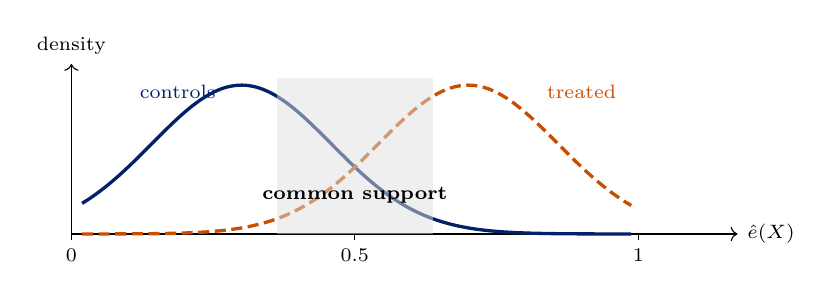
\begin{tikzpicture}[scale=0.9]
  \draw[->] (0,0) -- (9.4,0) node[right]{\scriptsize $\hat e(X)$};
  \draw[->] (0,0) -- (0,2.4) node[above]{\scriptsize density};
  \foreach \t/\lab in {0/0, 4/0.5, 8/1} \draw (\t,0) -- (\t,-0.08) node[below]{\scriptsize \lab};
  \draw[dukeblue,very thick,smooth,samples=80,domain=0.15:7.9,variable=\x]
    plot ({\x},{2.1*exp(-((\x-2.4)^2)/3.2)});
  \draw[accent,very thick,dash pattern=on 4pt off 2pt,smooth,samples=80,domain=0.15:7.9,variable=\x]
    plot ({\x},{2.1*exp(-((\x-5.6)^2)/3.2)});
  \node[dukeblue] at (1.5,2.0) {\scriptsize controls};
  \node[accent] at (7.2,2.0) {\scriptsize treated};
  \fill[gray!25,opacity=.5] (2.9,0) rectangle (5.1,2.2);
  \node at (4.0,0.55) {\scriptsize \textbf{common support}};
\end{tikzpicture}
\end{center}
\vskip-6pt
\begin{itemize}\itemsep2pt
  \item \textbf{Trim} to a range of $\hat e$ (say $[0.1,0.9]$), and say so. You
        have changed the estimand to that subpopulation.
  \item \textbf{Redefine the population} to the region where comparison is
        possible, often the honest and more interesting move.
  \item \textbf{Change the estimand}: the ATT needs overlap only for the treated;
        the ``overlap-weighted'' estimand \srcp{Li, Morgan, and Zaslavsky 2018}
        deliberately targets the region where comparison is best.
\end{itemize}
\end{frame}


%%%%%%%%%%%%%%%%%%%%%%%%%%%%%%%%%%%%%%%%%%%%%%%%%%%%%%%%%%%%%%%%%%%%%%%%%%%%%%%
\section[Weighting]{Weighting and G-Computation}
%%%%%%%%%%%%%%%%%%%%%%%%%%%%%%%%%%%%%%%%%%%%%%%%%%%%%%%%%%%%%%%%%%%%%%%%%%%%%%%
\begin{frame}\sectionpage\end{frame}

\begin{frame}{Inverse Probability Weighting}
Rare treated units in a covariate cell should count for more, because they stand
in for everyone like them who was not treated. Weight each unit by the inverse of
the probability of the treatment it actually received:
\begin{align*}
  \boxed{\;\hat\tau_{\text{IPW}}
  = \frac1n\sum_{i=1}^n \left[\frac{D_i Y_i}{\hat e(X_i)}
  - \frac{(1-D_i)Y_i}{1-\hat e(X_i)}\right]\;}
\end{align*}
\pause
\textbf{Why it works.} For the treated arm, condition on $X_i$ first:
\begin{align*}
  \E\!\left[\frac{D_i Y_i}{e(X_i)}\right]
  = \E\!\left[\frac{\E[D_i\mid X_i]\,\E[Y_i(1)\mid X_i]}{e(X_i)}\right]
  = \E\big[\E[Y_i(1)\mid X_i]\big] = \E[Y_i(1)] ,
\end{align*}
where ignorability lets us factor $D_i$ apart from $Y_i(1)$ given $X_i$, and
consistency replaces $Y_i$ by $Y_i(1)$ among the treated. Same for the control
arm. $\blacksquare$
\vskip2pt
This is the Horvitz--Thompson estimator from survey sampling, applied to a
``sample'' created by the treatment assignment mechanism.
\end{frame}

\begin{frame}[allowframebreaks,t]{One Class of Estimands, Three Members}
\srct{Hirano, Imbens, and Ridder (2003)}: IPW for the ATE, IPW for the ATT, and
the regression estimand are all members of one weighted-average family,
\begin{align*}
  \E\left[\,g(X_i)\left(\frac{Y_iD_i}{e(X_i)} - \frac{Y_i(1-D_i)}{1-e(X_i)}\right)\right] ,
\end{align*}
differing only in the choice of $g(\cdot)$:
\begin{center}\small
\renewcommand{\arraystretch}{1.7}
\begin{tabular}{ll}
\toprule
Estimand & $g(X_i)$ \\
\midrule
ATE & $1$ \\
ATT & $\dfrac{e(X_i)}{\Pr(D_i = 1)}$ \\
Regression & $\dfrac{e(X_i)\big(1-e(X_i)\big)}{\E\big[e(X_i)(1-e(X_i))\big]}$ \\
\bottomrule
\end{tabular}
\end{center}
\vskip2pt
\alert{This is the same anatomy result again}, now written as a weighting
function. Regression is not an alternative to weighting; it is a particular
weighting you did not choose.
\end{frame}

\begin{frame}{Stabilized IPW}
The raw weights $1/\hat e$ explode as $\hat e \to 0$: one observation with
$\hat e = 0.001$ carries the weight of a thousand. Multiply by the marginal
treatment probabilities:
\begin{align*}
  w_i^{\text{SIPW}} =
  \begin{cases}
    \dfrac{\Pr(D_i=1)}{e(X_i)}, & D_i = 1 \\[8pt]
    \dfrac{\Pr(D_i=0)}{1-e(X_i)}, & D_i = 0 .
  \end{cases}
\end{align*}
\pause
The rescaling cancels in the ratio, so the estimand is unchanged:
\begin{align*}
  \frac{\E\!\left[\frac{\Pr(D_i=1)}{e(X_i)}D_iY_i\right]}
       {\E\!\left[\frac{\Pr(D_i=1)}{e(X_i)}D_i\right]}
  = \frac{\E\!\left[\frac{1}{e(X_i)}D_iY_i\right]}
         {\E\!\left[\E\!\left[\frac{1}{e(X_i)}D_i \,\middle|\, X_i\right]\right]}
  = \E\!\left[\frac{D_iY_i}{e(X_i)}\right] = \E[Y_i(1)] ,
\end{align*}
because the denominator is $\E[e(X_i)/e(X_i)] = 1$.
\end{frame}

\begin{frame}[allowframebreaks,t]{Horvitz--Thompson versus H\'ajek}
The variance gain comes from \emph{normalizing}, not from the constant. Compare
a raw average with a ratio:
\begin{align*}
  \hat\delta_{\text{SIPW}}
  = \frac{\sum_i w_i^{\text{SIPW}} D_i Y_i}{\sum_i w_i^{\text{SIPW}} D_i}
  - \frac{\sum_i w_i^{\text{SIPW}} (1-D_i) Y_i}{\sum_i w_i^{\text{SIPW}}(1-D_i)} .
\end{align*}
\vskip3pt
\begin{itemize}\itemsep2pt
  \item \alert{Note the arithmetic}: the constant $\Pr(D_i=1)$ appears in both
        numerator and denominator of the ratio and \emph{cancels}. So for this
        estimator, ``stabilizing'' changes nothing; what matters is that we divided
        by $\sum_i w_i$ rather than by $n$.
  \item That normalization is the real gain. The H\'ajek estimator's weights sum
        to the sample size in each arm, so the weighted pseudo-population is not
        artificially inflated, the estimate respects the range of $Y$, and its
        variance is typically much smaller.
  \item Stabilized weights \emph{do} matter when the weights enter a regression
        rather than a ratio, the marginal structural model setting.
  \item \alert{Neither fixes poor overlap.} Extreme weights survive both; they
        are a positivity problem wearing a disguise. Diagnose with the largest
        weights and the \emph{effective sample size}
        $\big(\sum_i w_i\big)^2/\sum_i w_i^2$.
\end{itemize}
\end{frame}

\begin{frame}[allowframebreaks,t]{IPW Is a Weighted Regression}
Define the \alert{Horvitz--Thompson transformation}
\begin{align*}
  H_i = \frac{D_i}{e(X_i)} - \frac{1-D_i}{1-e(X_i)} .
\end{align*}
Then $\E[H_i Y_i] = \E[Y_i(1)-Y_i(0)]$, which is the IPW estimand written in one
term. Equivalently:
\vskip3pt
\begin{block}{}
The coefficient on $D_i$ from a \textbf{weighted least squares} regression of
$Y_i$ on $D_i$ (with an intercept) and weights $1/\hat e(X_i)$ for the treated,
$1/(1-\hat e(X_i))$ for the controls, equals the \emph{normalized} (H\'ajek) IPW
estimator, a difference in weighted means. It is not the raw
Horvitz--Thompson average, which divides by $n$ instead.
\end{block}
\vskip3pt
\begin{itemize}\itemsep2pt
  \item Practically convenient: you can run IPW with \texttt{lm(y \textasciitilde\ d,
        weights = w)} and add covariates for extra protection.
  \item Conceptually important: it makes the continuity between ``weighting'' and
        ``regression'' explicit, and it is the bridge to the doubly robust
        estimator below.
  \item Note the standard errors from \texttt{lm} will be wrong, they ignore
        that $\hat e$ was estimated. Bootstrap the whole pipeline.
\end{itemize}
\end{frame}

\begin{frame}[allowframebreaks,t]{Weighting to Different Estimands}
Every adjustment method is a choice of weights on covariate cells. Writing them
side by side makes the choice explicit:
\begin{center}\small
\renewcommand{\arraystretch}{1.55}
\begin{tabular}{lll}
\toprule
Estimand & Weight on treated & Weight on controls \\
\midrule
ATE & $1/e(X)$ & $1/(1-e(X))$ \\
ATT & $1$ & $e(X)/(1-e(X))$ \\
ATU & $(1-e(X))/e(X)$ & $1$ \\
Overlap (ATO) & $1-e(X)$ & $e(X)$ \\
\bottomrule
\end{tabular}
\end{center}
\vskip4pt
\begin{itemize}\itemsep2pt
  \item The ATT weights leave the treated alone and reweight controls to look
        like them, which is what ``the effect on the treated'' means.
  \item The \emph{overlap} weights are bounded and largest at $e = 0.5$; they
        never explode. Note that they reproduce exactly the regression weighting
        $e(x)(1-e(x))$ from the anatomy, so ``ATO'' is the estimand OLS was
        targeting all along, now chosen deliberately
        \srcp{Li, Morgan, and Zaslavsky 2018}.
\end{itemize}
\end{frame}

\begin{frame}[allowframebreaks,t]{G-Computation: the Other Half}
Instead of modelling treatment, model the outcome. Under ignorability and common
support, fit
\begin{align*}
  m_d(x) = \E[Y_i \mid D_i = d, X_i = x], \qquad d\in\{0,1\} ,
\end{align*}
then \emph{impute both potential outcomes for everyone} and average:
\begin{align*}
  \hat\tau_{\text{g-comp}} = \frac1n\sum_{i=1}^n
  \big[\hat m_1(X_i) - \hat m_0(X_i)\big] .
\end{align*}
\begin{itemize}\itemsep2pt
  \item This is exactly the ``observed-value'' predicted-probability procedure
        from Week 4, and in the linear case it \emph{is} regression adjustment.
  \item It uses the whole sample and is efficient when the outcome model is
        right. It \alert{extrapolates silently} when it is not: $\hat m_1(x)$ is
        computed even for $x$ where nobody was treated.
  \item Note the symmetry: IPW models $\Pr(D\mid X)$ and never touches $Y$;
        g-computation models $\E[Y\mid D,X]$ and never touches assignment.
        Each is exposed to a different misspecification, which is the opening
        for the next section.
\end{itemize}
\end{frame}

%%%%%%%%%%%%%%%%%%%%%%%%%%%%%%%%%%%%%%%%%%%%%%%%%%%%%%%%%%%%%%%%%%%%%%%%%%%%%%%
\section[Doubly Robust]{Doubly Robust Estimation}
%%%%%%%%%%%%%%%%%%%%%%%%%%%%%%%%%%%%%%%%%%%%%%%%%%%%%%%%%%%%%%%%%%%%%%%%%%%%%%%
\begin{frame}\sectionpage\end{frame}

\begin{frame}{Why Not Both?}
IPW is consistent only if $e(X_i)$ is right. G-computation is consistent only if
$m_d(X_i)$ is right. Combine them so that \emph{either} suffices.
\vskip3pt
Given the two nuisance functions
$m_d(x) = \E[Y_i\mid D_i=d,X_i=x]$ and $e(x) = \Pr(D_i=1\mid X_i=x)$, the
\alert{augmented IPW} estimand is
\begin{align*}
  \theta = \E\Bigg[
  \underbrace{m_1(X_i) - m_0(X_i)}_{\text{g-computation}}
  + \underbrace{\frac{D_i\big(Y_i - m_1(X_i)\big)}{e(X_i)}
  - \frac{(1-D_i)\big(Y_i-m_0(X_i)\big)}{1-e(X_i)}}_{\text{IPW-weighted residuals}}
  \Bigg]
\end{align*}
\vskip3pt
\begin{block}{Double robustness}
$\theta = \E[Y_i(1)-Y_i(0)]$ if \alert{either} $m_d$ \alert{or} $e$ is correctly
specified, not necessarily both. And when both are right, AIPW attains the
semiparametric efficiency bound.
\end{block}
\end{frame}

\begin{frame}{Case 1: the Outcome Model Is Correct}
Suppose $m_1$ is right but $e$ is arbitrary. Look at the augmentation term for
the treated arm, conditioning on $X_i$:
\begin{align*}
  \E\!\left[\frac{D_i}{e(X_i)}\big(Y_i - m_1(X_i)\big)\ \middle|\ X_i\right]
  &= \frac{1}{e(X_i)}\,\Pr(D_i=1\mid X_i)\,
     \E\big[Y_i - m_1(X_i)\mid D_i=1,X_i\big] \\[2pt]
  &= \frac{1}{e(X_i)}\,\E[D_i \mid X_i]\cdot \underbrace{0}_{\text{by definition of } m_1}
   \;=\; 0 .
\end{align*}
\pause
The same argument gives
$\E\big[\tfrac{1-D_i}{1-e(X_i)}(Y_i - m_0(X_i)) \mid X_i\big] = 0$. Hence
\begin{align*}
  \theta = \E\big[m_1(X_i) - m_0(X_i)\big] = \E[Y_i(1)-Y_i(0)] .
\end{align*}
\vskip2pt
\alert{The whole augmentation term vanishes}, whatever $e$ is. Note that this
did not use a correct propensity score anywhere.
\end{frame}

\begin{frame}{Case 2: the Propensity Score Is Correct}
Now suppose $e$ is right but $m_1$ is some wrong function. Then
\begin{align*}
  \E\!\left[\frac{D_i}{e(X_i)}\big(Y_i - m_1(X_i)\big)\ \middle|\ X_i\right]
  = \frac{1}{e(X_i)}\E[D_iY_i\mid X_i] - m_1(X_i) .
\end{align*}
Since $\E[D_iY_i\mid X_i] = e(X_i)\,\E[Y_i(1)\mid X_i]$ by ignorability, this is
\begin{align*}
  \E[Y_i(1)\mid X_i] - m_1(X_i) .
\end{align*}
\pause
Symmetrically the control term contributes
$-\big(\E[Y_i(0)\mid X_i] - m_0(X_i)\big)$. Adding everything up, the wrong
$m_1, m_0$ cancel exactly:
\begin{align*}
  \theta = \E\Big[\E[Y_i(1)\mid X_i] - \E[Y_i(0)\mid X_i]\Big]
         = \E[Y_i(1)-Y_i(0)] . \qquad\blacksquare
\end{align*}
\vskip2pt
Two independent routes to the same answer. That is the insurance.
\end{frame}

\begin{frame}{Why the Cancellation Matters Beyond This Week}
Look again at what happened in the two cases. A first-order error in \emph{one}
nuisance function was wiped out by the other term. That is not a coincidence of
AIPW; it is a property the estimating equation was built to have.
\vskip4pt
\begin{block}{The consequence}
The bias of AIPW is roughly the \emph{product} of the two nuisance errors, not
their sum. So if both $\hat e$ and $\hat m_d$ are merely \emph{approximately}
right, the bias is second-order small, much smaller than either model's own
error.
\end{block}
\vskip4pt
\begin{itemize}\itemsep3pt
  \item This is why doubly robust estimators are the default in modern practice
        even when nobody believes either model exactly.
  \item It is also what eventually licenses estimating $\hat e$ and $\hat m_d$
        with flexible, machine-learning methods rather than logit and OLS.
        \alert{That is a Week 13 topic}; the property has a name (\emph{Neyman
        orthogonality}) and we will not need it before then.
\end{itemize}
\end{frame}

\begin{frame}{An Honest Warning}
Double robustness is often oversold.
\vskip3pt
\begin{itemize}\itemsep2pt
  \item ``Either model correct'' is a low bar in theory and an unreachable one in
        practice: both models are almost certainly wrong, and then AIPW is
        inconsistent too.
  \item What it really buys is \alert{second-order bias}: the bias is the
        \emph{product} of the two models' errors, so it is small when both are
        approximately right. That is genuinely valuable, and it is the honest
        version of the claim.
  \item With extreme weights, AIPW can be more unstable than either component
        alone \srcp{Kang and Schafer 2007}.
  \item \alert{None of this addresses unobserved confounding.} Everything today
        assumes conditional ignorability, and no diagnostic can test it.
\end{itemize}
\end{frame}

\begin{frame}{Sensitivity Analysis: Taking the Assumption Seriously}
Since ignorability is untestable, ask instead: \emph{how strong would an
unobserved confounder have to be to overturn my conclusion?}
\vskip3pt
\begin{itemize}\itemsep3pt
  \item \textbf{Rosenbaum bounds}: how much would two matched units have to
        differ in their odds of treatment before the inference flips?
  \item \textbf{Partial $R^2$ / robustness value} \srcp{Cinelli and Hazlett 2020}:
        express the required confounder strength as the share of residual
        variation in $D$ and in $Y$ it would have to explain, then benchmark it
        against an \emph{observed} covariate, ``the confounder would need to
        be three times as strong as parental education.''
  \item \textbf{$E$-value}: the minimum risk ratio a confounder would need with
        both treatment and outcome.
\end{itemize}
\vskip3pt
\alert{Report one.} It converts an untestable assumption into a quantitative
claim your reader can argue with.
\end{frame}

\begin{frame}[allowframebreaks,t]{Choosing Among the Methods}
\begin{center}\footnotesize
\renewcommand{\arraystretch}{1.2}
\begin{tabular}{lll}
\toprule
Method & Models & Main weakness \\
\midrule
Exact / CEM matching & nothing & discards data; infeasible with many covariates \\
NN / Mahalanobis matching & a distance & bias with continuous $X$; variance from reuse \\
PS matching & $\Pr(D\mid X)$ & sensitive to the PS model; discards controls \\
IPW & $\Pr(D\mid X)$ & extreme weights when overlap is poor \\
Regression / g-computation & $\E[Y\mid D,X]$ & silent extrapolation; own weighting \\
AIPW & both & unstable weights; still needs ignorability \\
\bottomrule
\end{tabular}
\end{center}
\vskip4pt
\begin{itemize}\itemsep2pt
  \item \alert{If the answers differ a lot, that is worth chasing down.} By the
        anatomy results, systematic differences can mean the cell-level effects
        $\delta(x)$ are heterogeneous and the methods weight them differently, 
        but they can equally reflect a misspecified model, poor overlap, or
        sampling noise. Distinguish these before concluding anything.
  \item Report the primary estimator you pre-committed to, plus the others as
        robustness, never the reverse.
\end{itemize}
\end{frame}

\begin{frame}{A Workflow}
\begin{enumerate}\itemsep2pt
  \item State the estimand (ATE? ATT? ATO? on which population?) before touching
        data.
  \item Draw the DAG. Decide what to condition on, and what \emph{not} to.
  \item Estimate the propensity score. Look at overlap. Trim or redefine if needed
        and say so.
  \item Match or weight. Check balance with standardized mean differences and
        density plots, \alert{never} with $t$-tests.
  \item Estimate with a doubly robust estimator; report matching, weighting, and
        regression alongside.
  \item Get standard errors that respect the design: bootstrap the whole
        estimation pipeline for weighting and regression estimators, and cluster
        where treatment was assigned. \alert{Do not bootstrap nearest-neighbour
        matching}, the ordinary bootstrap is invalid for it
        \srcp{Abadie and Imbens 2008}; use their analytic variance instead.
  \item Report a sensitivity analysis.
\end{enumerate}
\end{frame}

\begin{frame}[allowframebreaks,t]{Looking Ahead}
\begin{itemize}\itemsep4pt
  \item Everything today rested on \alert{conditional ignorability}: the claim
        that we measured every confounder. Matching, weighting, and AIPW make
        that assumption easier to implement; they do not make it more likely
        to be true.
  \item The anatomy results are the transferable lesson: \emph{every} adjustment
        method is a weighting of cell-level effects, and knowing the weights tells
        you what your number means.
  \item \textbf{Weeks 7--11} abandon ignorability and look for special structure
 (an instrument, a discontinuity, parallel trends) that identifies an
        effect \emph{despite} unobserved confounding.
  \item \textbf{Week 13} returns to today's AIPW estimator and asks what changes
        when the covariate set is large enough that logit and OLS will not do.
\end{itemize}
\vskip3pt
\begin{block}{Problem Set 3}
Assigned today, due Monday October 12. Covers Weeks 5--6.
\end{block}
\end{frame}

\begin{frame}[allowframebreaks,t]{References}
\footnotesize
\begin{itemize}\itemsep3pt
\item Abadie, Alberto and Guido W. Imbens. 2008. ``On the Failure of the
Bootstrap for Matching Estimators.'' \textit{Econometrica} 76(6): 1537--1557.
\item Angrist, Joshua D. 1998. ``Estimating the Labor Market Impact of Voluntary
Military Service Using Social Security Data on Military Applicants.''
\textit{Econometrica} 66(2): 249--288.
\item Cinelli, Carlos and Chad Hazlett. 2020. ``Making Sense of Sensitivity:
Extending Omitted Variable Bias.'' \textit{Journal of the Royal Statistical
Society B} 82(1): 39--67.
\item Ho, Daniel E., Kosuke Imai, Gary King, and Elizabeth A. Stuart. 2007.
``Matching as Nonparametric Preprocessing for Reducing Model Dependence in
Parametric Causal Inference.'' \textit{Political Analysis} 15(3): 199--236.
\item Imai, Kosuke, Gary King, and Elizabeth A. Stuart. 2008. ``Misunderstandings
Between Experimentalists and Observationalists About Causal Inference.''
\textit{Journal of the Royal Statistical Society A} 171(2): 481--502.
\item Hirano, Keisuke, Guido W. Imbens, and Geert Ridder. 2003. ``Efficient
Estimation of Average Treatment Effects Using the Estimated Propensity Score.''
\textit{Econometrica} 71(4): 1161--1189.
\item Kang, Joseph D.Y. and Joseph L. Schafer. 2007. ``Demystifying Double
Robustness.'' \textit{Statistical Science} 22(4): 523--539.
\item Li, Fan, Kari Lock Morgan, and Alan M. Zaslavsky. 2018. ``Balancing
Covariates via Propensity Score Weighting.'' \textit{Journal of the American
Statistical Association} 113(521): 390--400.
\item Morgan, Stephen L. and Christopher Winship. 2015.
\textit{Counterfactuals and Causal Inference}, 2nd ed. Cambridge University
Press. [Ch.\ 4, 5, 7, 8]
\item Rosenbaum, Paul R. and Donald B. Rubin. 1983. ``The Central Role of the
Propensity Score in Observational Studies for Causal Effects.''
\textit{Biometrika} 70(1): 41--55.
\item Sekhon, Jasjeet S. 2009. ``Opiates for the Matches: Matching Methods for
Causal Inference.'' \textit{Annual Review of Political Science} 12: 487--508.
\end{itemize}
\end{frame}

\end{document}
